%%Politecnico di Bari - Department of Electrical and Information Engineering
%%Electronics for Telecommunications Laboratory (ETLCLab)
%%TeX Template for ETLCLab Thesis
%%Author: Antonello Florio, MSc
%%Rev 0.1 - Dec2021

\documentclass[a4paper,12pt,oneside]{book}
%%Language and encoding
\usepackage [english]{varioref}
\usepackage[T1]{fontenc}
\usepackage[utf8]{inputenc}
\usepackage[english]{babel}
%%Margins
\usepackage[a4paper,top=2.5cm,bottom=2.5cm,left=3.5cm,right=2.5cm]{geometry}

%% List of useful packages 
\usepackage{setspace}
\onehalfspacing
\usepackage{amsmath,amssymb,amsthm} 
\usepackage{emptypage}
\usepackage{graphicx}
\usepackage{booktabs}
\usepackage[table]{ xcolor }
\usepackage{caption}
\captionsetup{font=scriptsize, format=hang, labelfont={sf,bf}}
\usepackage{mathtools}
\usepackage{amsmath}
\usepackage{subfig}
\usepackage[]{algorithm}
\usepackage{algorithmic}
\usepackage{siunitx}
\usepackage[italian=guillemets]{csquotes}
\usepackage{hyperref}
\hypersetup{hidelinks}
\makeatletter

%%Absolute value with \left|-\right|
\newcommand\abs{\@ifstar\lr@abs\n@abs}
\newcommand\lr@abs[1]{\left|#1\right|}
\newcommand\n@abs[2][]{\mathopen{#1|}#2\mathclose{#1|}}

\makeatother
\usepackage{pdfpages}


%%Bibliography with biblatex
\usepackage[backend=bibtex,style=ieee,sorting=none]{biblatex}
\bibliography{bib/bibl_tesi}{}

%%Style setting for equations (reset for each chapter)
\numberwithin{equation}{chapter}
%\input{misc/glossary}

\begin{document}
	\frontmatter
	%%Include disclaimer
	%\includepdf[pages=-]{misc/liberatoria_tesi.pdf}
	%%Include frontpage
	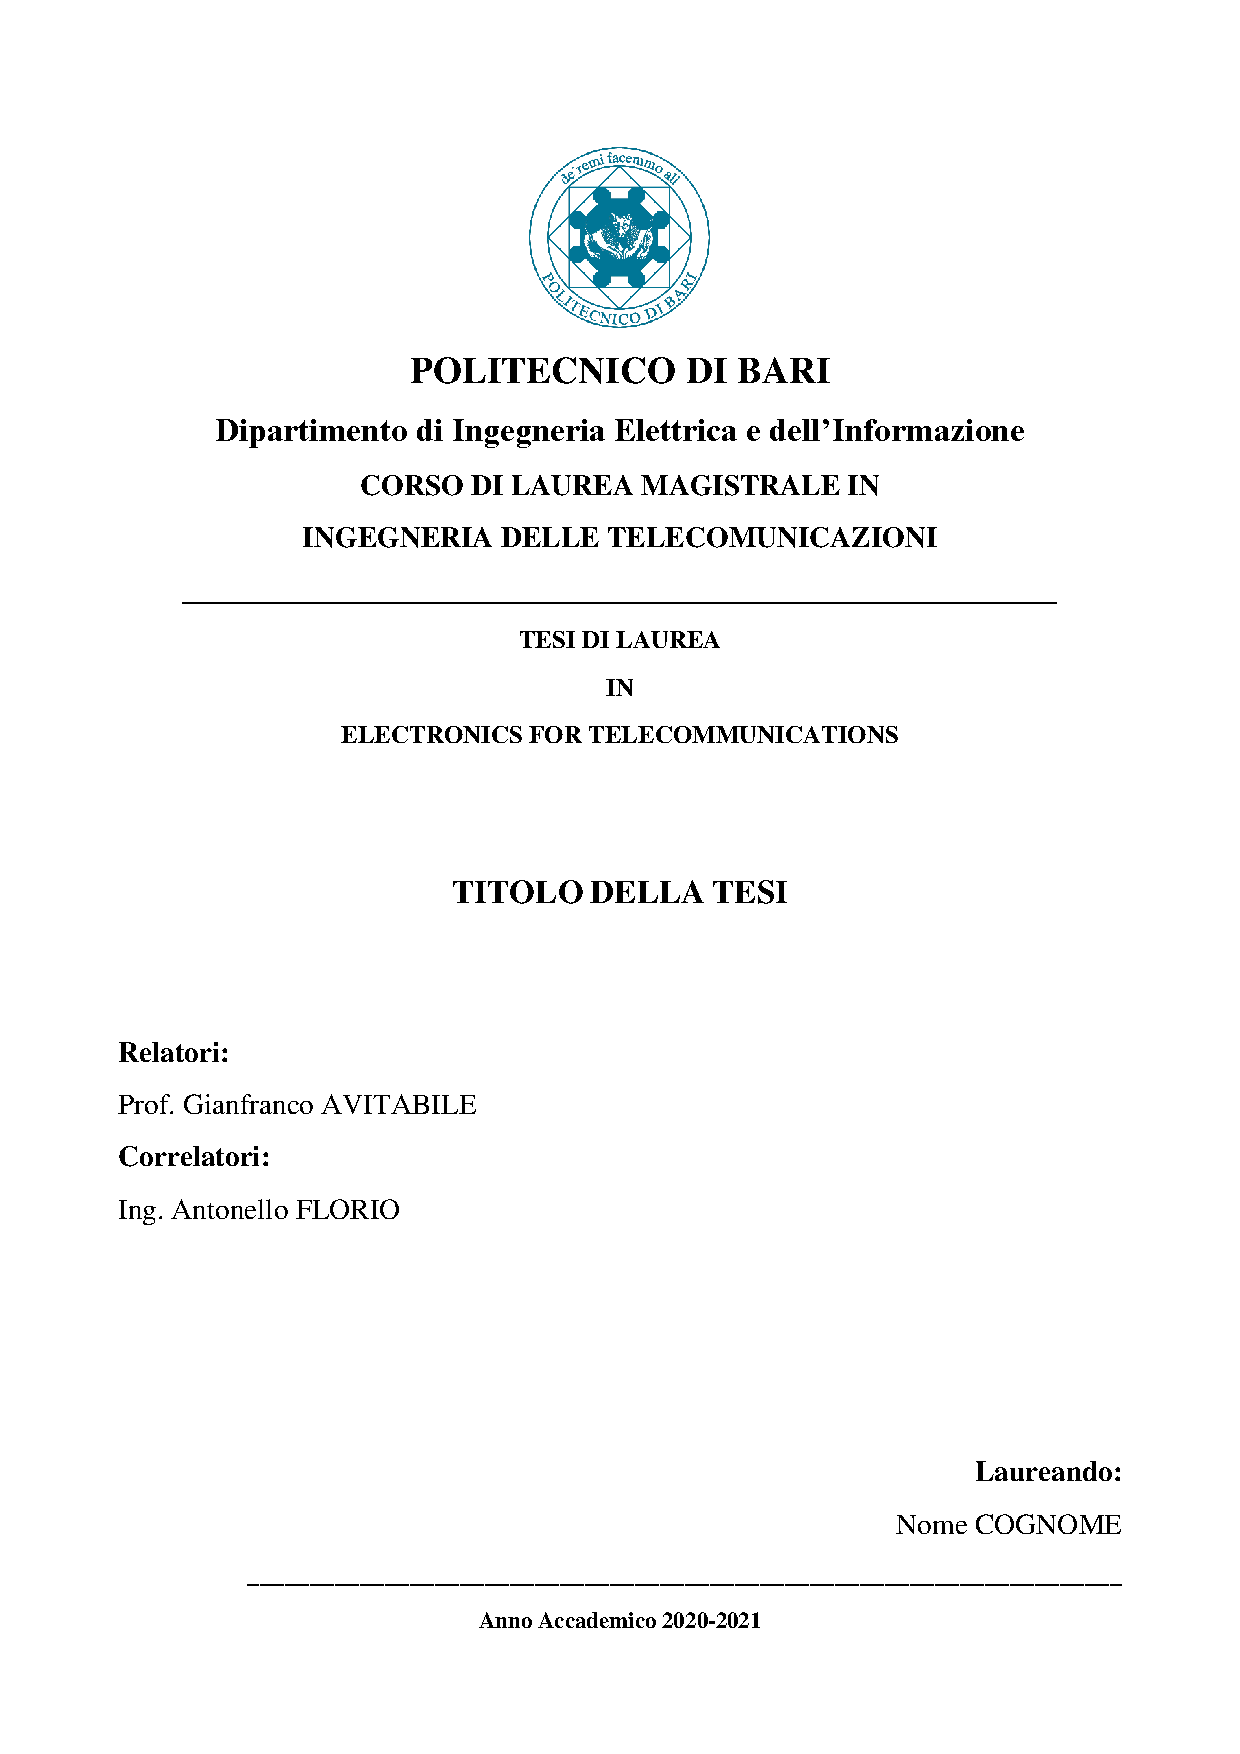
\includepdf[pages=-]{misc/Frontespizio.pdf}
	\shipout\null
	%%Miscellaneous
	\addcontentsline{toc}{chapter}{Summary}
\chapter*{Summary}
\label{Abstract}
Abstract should go here

	\tableofcontents
	\listoffigures
\listoftables
	\mainmatter
	%%Sourcing chapters
	\chapter{Chapter 1}\label{chap:chapter1}

Text goes here

\section{Section tile}
You can handle sections \cite{music}
\subsection{Subsection title}
And also subsections :-)
	\backmatter
	%%References
	\addcontentsline{toc}{chapter}{References}
	\printbibliography
	%%Acknowledgements
	%\input{misc/ringraziamenti}
\end{document}

	